\chapter{Introduction}
Protoplanetary disks are planet-forming, potentially planet-containing, dust- and gas-rich disks around young stars. Disk chemistry also provides some of our best tools to characterize disk structures and dynamics, including the presence of protoplanets. Developing a predictive theory of planet formation therefore requires a deep understanding of the chemistry of protoplanetary disks (Oberg21).

Protoplanetary disks emerge within the context of star formation, when infalling interstellar cloud material becomes distributed in disk-like structures to preserve angular momentum (Shun87). It is a gradual process which involves multiple stages like the interstellar phase, the protostellar phase and finally the disk phase. The inheritance of chemical compositions across these phases is of immense importance as it is carried till formation of first planets as well.




\begin{figure}
	\centering
	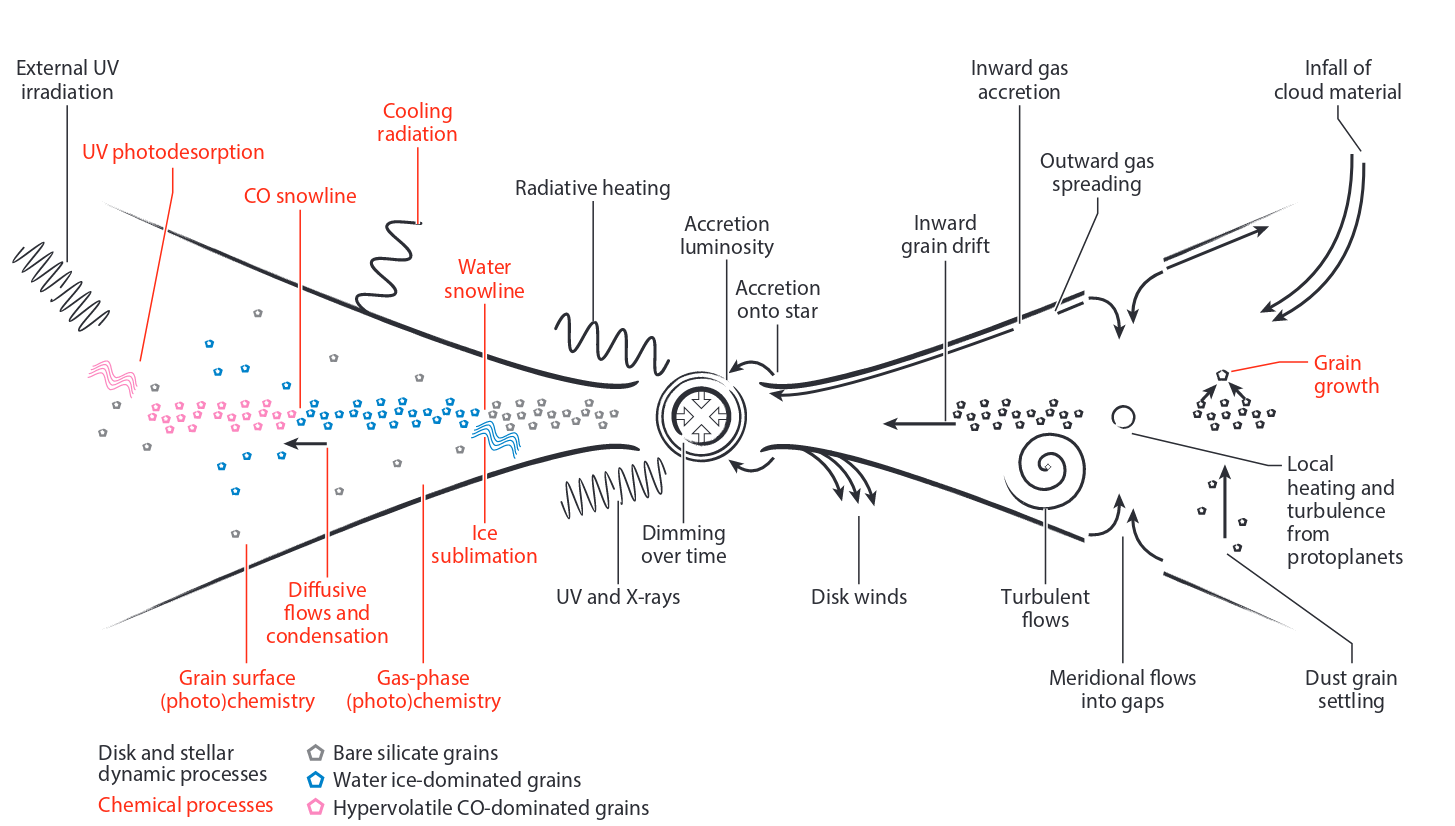
\includegraphics[angle=90, width=0.8\linewidth]{screenshot002}
	\caption{An overview of different physical and chemical processes that go in
	protoplanetary disks. The processes labelled in black are stellar and/or disk
	dynamical processes which do not depend on local chemical environment. Processes
	labelled in red are the chemistry dependent mechanisms.}
	\label{fig:screenshot002}
\end{figure}

